\documentclass[10pt,letterpaper]{article}
\usepackage{enumitem}
\usepackage[utf8]{inputenc}
\usepackage[spanish]{babel}
\usepackage{graphicx}
\usepackage{amsmath}
\usepackage{amsfonts}
\usepackage{amssymb}
\usepackage{makeidx}
\usepackage{graphicx}
\usepackage{url}
\usepackage{hyperref}
\usepackage{minted}
\usepackage[dvipsnames]{xcolor}
\usepackage[left=2cm,right=2cm,top=1.5cm,bottom=1.5cm]{geometry}
\usepackage{biblatex}
\addbibresource{Bib.bib}

\begin{document}

\thispagestyle{empty}
	
	\begin{figure}[ht]
	   \minipage{0.76\textwidth}
			\includegraphics[width=4cm]{Proyecto/IMAGES/Logo_UNAM.png}
			\label{EscudoUNAM}
	   \endminipage
	   \minipage{0.32\textwidth}
			\includegraphics[height = 4.9cm ,width=4cm]{Proyecto/IMAGES/Logo_FC.png}
			\label{EscudoFC}
		\endminipage
	\end{figure}
	
	\begin{center}
	\vspace{0.8cm}
	\LARGE
	UNIVERSIDAD NACIONAL AUTÓNOMA DE MÉXICO 
	
	\vspace{0.8cm}
	\LARGE
	FACULTAD DE CIENCIAS
	
	\vspace{.5cm}	
	\Large
	\textbf{Práctica 2}

	\vspace{.7cm}
	\normalsize	
	EQUIPO \\
	\vspace{.3cm}
	\large
	\textbf{Arroyo Martínez Erick Daniel} \\ 
    \textbf{Terrazas Rivera Alex}\\
    \textbf{Vergara Navarro Mixtli Arturo}
	\vspace{.7cm}\\
	\normalsize	
	PROFESOR \\
	\vspace{.3cm}
	\large
	\textbf{Gilde Valeria Rodríguez Jiménez}

    \vspace{.7cm}
	\normalsize	
	AYUDANTES \\
	\vspace{.3cm}
	\large
	\textbf{Rogelio Alcantar Arenas}\\
    \textbf{Gibran Aguilar Zuñiga}\\
    \textbf{Luis Angel Leyva Castillo}\\
    \textbf{Rogelio Alcantar Arenas}
	
	\vspace{.7cm}
	\normalsize	
	ASIGNATURA \\
	\vspace{.3cm}
	\large
	\textbf{Computación Concurrente}
	
	\vspace{.2cm}
	\today
	\end{center}
	\newpage

%%% Indice
%\tableofcontents
%\newpage

\subsection*{Gráficas y tablas de valores}  

\begin{itemize}
    \item[A] 1 Hilo

    \item[B] 2 Hilos

    \item[C] 27 Hilos

    \item[D] 100 Hilos
\end{itemize}

\begin{figure}[H]
    \centering
    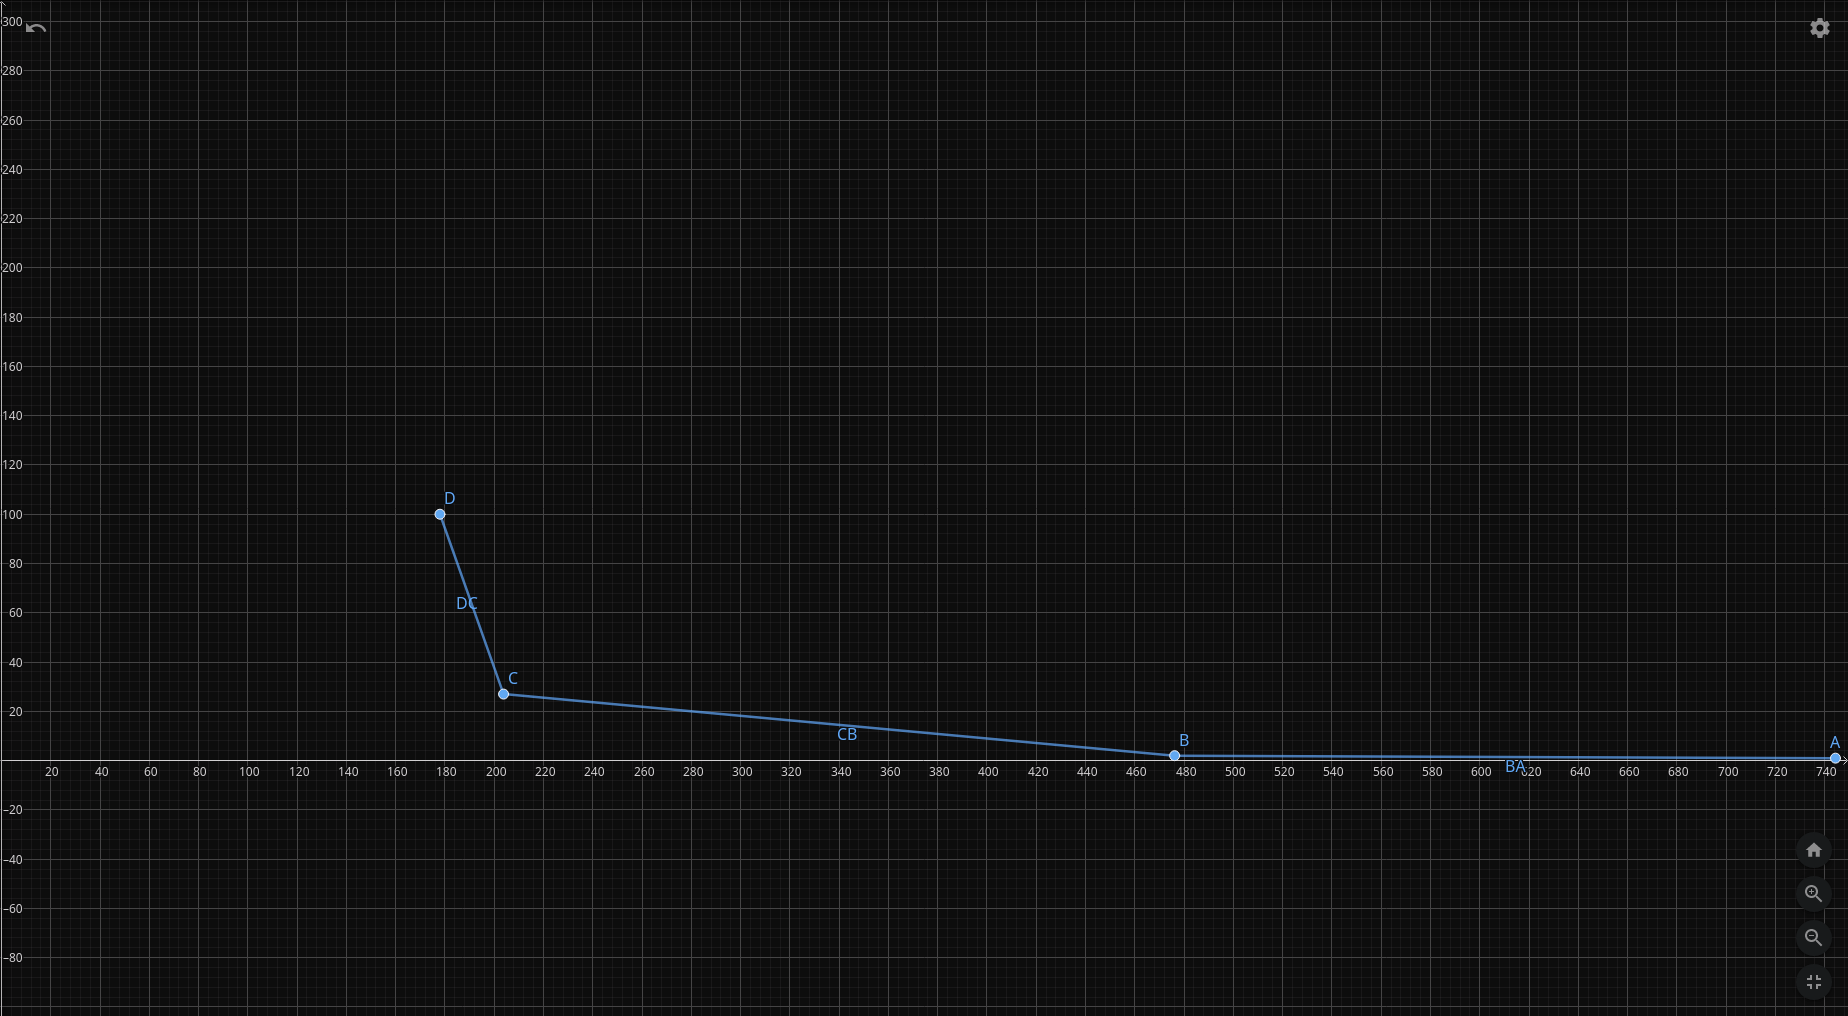
\includegraphics[scale=0.29]{P02/IMG/00.png}
\end{figure}

\begin{center}
    \begin{tabular}{|c|c|c|c|}
         \hline
         \# Hilos & Aceleración Teórica & Aceleración Obtenida & \% Código en Paralelo\\
         \hline
         1 & 1 & 1 & 80\\
         \hline
         2 & 1.6666666666667 & 1.56330408558 & 80\\
         \hline
         27 & 4.3548387096774 & 3.65276489668 & 80\\
         \hline
         100 & 4.8076923076923 & 4.18255475519 & 80\\
         \hline
    \end{tabular}
\end{center}

\subsection*{Mensaje Descifrado}

    \begin{figure}[H]
        \centering
        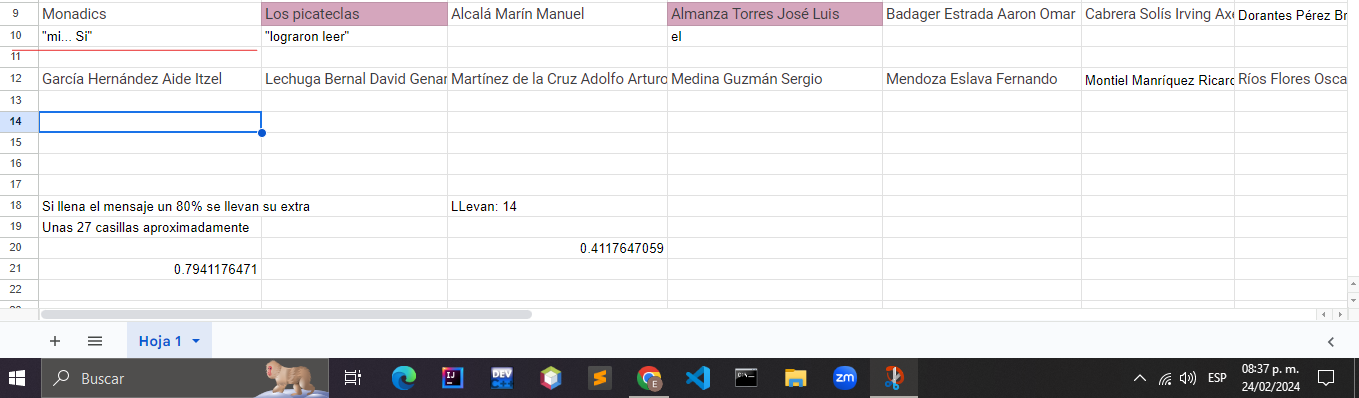
\includegraphics[scale=0.5]{P02/IMG/20240224-WA0002.png}
        \caption{Captura de pantalla cuando se agregó la palabra}
        \label{fig:}
    \end{figure}


\subsection*{Cuestionario}
    
    \begin{itemize}
        \item ¿Cuál fue mi contraseña?

        "mndics"

        \item ¿Cuantas posibles contraseñas hay?

        El posible número de contraseñas con seis caracteres es 736,281

        \item ¿La ley de Amdahl siempre se cumple?

        No siempre se cumple.

        \item ¿En que casos no se cumple?

        Cuándo el tiempo de comunicación del equipo es muy lento, por ejemplo tener un CPU muy nuevo mientras que todos los demás componentes son muy viejos o con el Load Balancing que puede dar más o menos recursos a una tarea determinada.

        \item ¿Por que crees a que se debe esto? 

        Porque la Ley de Amdahl no toma en cuenta estos diferentes factores y, por lo tanto, las predicciones que haga asumirán que los factores anteriores no afectan mucho al speedup lo cual no siempre es cierto.

        \item ¿Cual sería la mejora máxima? Es decir, la aceleración teórica máxima.

        La aceleración teórica máxima será de $4.9999\dots$

        \item Escribe tus conclusiones, además de lo que aprendiste en esta practica, contratiempos y descubrimientos que hubo durante su realización. 

        En esta práctica aprendimos de una manera práctica lo mucho que nos puede ayudar la paralización de un programa para resolver ciertos tipos de problemas, además observamos sus limitaciones en cuanto a la mejora de tiempo que este tipo de técnicas nos pueden brindar.

        También calculamos las mejoras teóricas con la Ley de Amdahl y logramos observar que no siempre se cumplen los valores exactos pero, aún así, sigue siendo una buena aproximación a la realidad de los datos.

        Se tuvieron pequeños problemas al principio de la práctica ya que nuestra contraseña era un poco larga, pero nos la cambiaron y todo salio bien.

        


        \item ¿Cuál es su rol?

        Nuestro rol es ser diferentes hilos ya que, al realizar diferentes procesos de manera simultanea, resolvimos una pequeña parte de un problema más grande que fue obtener cierta cantidad de palabras para poder completar el mensaje.

        \item ¿Cuál es mi rol?

        Tú rol fue ser el CPU, ya que organizaste a todos los equipos para asignarles un problema diferente a cada uno mientras verificabas el progreso de cada uno.


    \end{itemize}

%% Desarrollo
%% Referencias
%\printbibliography[heading=bibintoc, title={Referencias bibliográficas} ]
\end{document}